\documentclass[11pt,a4paper]{article}

\usepackage[margin=2.2cm]{geometry}
\usepackage{amsmath,amssymb}
\usepackage{graphicx}
\usepackage{xcolor}
\usepackage{booktabs}
\usepackage{listings}
\usepackage{pgfplots}
\usepackage{caption}
\usepackage[hidelinks]{hyperref}

\pgfplotsset{compat=1.18}
\graphicspath{{figures/}}

\definecolor{cWork}{RGB}{41,128,185}
\definecolor{cWait}{RGB}{230,126,34}
\definecolor{cComm}{RGB}{46,204,113}

\lstset{
    language=C,
    basicstyle=\ttfamily\footnotesize,
    keywordstyle=\bfseries\color{blue!70!black},
    commentstyle=\itshape\color{gray},
    numbers=left,
    numberstyle=\tiny\color{gray},
    numbersep=5pt,
    frame=single,
    breaklines=true,
    columns=flexible,
    showstringspaces=false,
    tabsize=4,
    morekeywords={MPI_Scatter,MPI_Gather,MPI_Barrier,MPI_Send,MPI_Recv,
        MPI_Isend,MPI_Irecv,MPI_Waitall,MPI_Status,MPI_Request,
        MPI_COMM_WORLD,MPI_INT,MPI_FLOAT,MPI_BYTE,MPI_ANY_SOURCE,
        MPI_ANY_TAG,MPI_STATUS_IGNORE,MPI_STATUSES_IGNORE,MPI_Wtime,
        MPI_Init,MPI_Finalize,MPI_Comm_rank,MPI_Comm_size,MPI_Abort},
    xleftmargin=1em,
    framexleftmargin=1em,
}

\newcommand{\tserial}{35.632}

\title{MPI Parallelisation of the Mandelbrot Set}
\author{}
\date{}

\begin{document}
\maketitle
\thispagestyle{empty}

%======================================================================
\section{Introduction}
%======================================================================

The Mandelbrot set is defined as the set of complex numbers $\kappa$ for
which the iterative sequence
\[
    z_{i+1} = z_i^2 + \kappa, \qquad z_0 = \kappa,
\]
remains bounded. Since the set is contained within $|\kappa| < 2$, it
suffices to iterate until $|z_i| > 2$ to classify a point as outside the
set, with an upper bound of $\texttt{MAXITER} = 1000$ iterations.

The serial implementation discretises the region
$-2 \le \operatorname{Re}(\kappa) \le 2$,\;
$-2 \le \operatorname{Im}(\kappa) \le 2$ on an $N \times N$ grid
($N = 15{,}000$) and records the iteration count at each pixel. The
Mandelbrot set is symmetric about the real axis
($\operatorname{Im}(\kappa) \to -\operatorname{Im}(\kappa)$), so
only the top half plus the middle row is computed---a total of
$H = (N/2+1) \times N = 112{,}515{,}000$ pixels---and the lower half is
obtained by mirroring. The iteration counts are converted to false colour
and written to a PPM image (Figure~\ref{fig:mandelbrot}).

\begin{figure}[h]
    \centering
    
\includegraphics[width=0.35\textwidth]{mandelbrot.png}
    \caption{Mandelbrot set rendered by the serial code at $N = 4000$.}
    \label{fig:mandelbrot}
\end{figure}

The serial code completes in \textbf{\tserial\,s} at $N = 15{,}000$. All
three MPI parallelisations below use $p = 10$ processes and the same
symmetry optimisation.

%======================================================================
\section{Task~1: Static Decomposition (Block Partitioning)}
\label{sec:task1}
%======================================================================

\subsection{Data Distribution and Algorithm}

The $H$ pixel indices are divided into $p = 10$ equal, contiguous blocks of
size $C = H / p = 11{,}251{,}500$. Rank~$r$ receives and processes
the block $[rC,\; (r{+}1)C)$. Because pixel indices are laid out
row-by-row, each block corresponds to a horizontal strip of
$\approx C/N \approx 750$ consecutive rows of the grid.

The root process initialises an array of sequential indices $0, 1, \ldots,
H{-}1$ and distributes them with \texttt{MPI\_Scatter}. Each rank computes
the iteration count for its assigned pixels using the standard escape-time
loop, then all results are collected at the root via \texttt{MPI\_Gather}.
Barriers before and after the computation delimit the timing regions.

\subsection{Key Code}
\begin{lstlisting}
int half = (N/2 + 1) * N;
int chunksize = half / n_ranks;

MPI_Scatter(n, chunksize, MPI_INT,
            _n, chunksize, MPI_INT, 0, MPI_COMM_WORLD);

for (loop = 0; loop < chunksize; loop++) {
    i = _n[loop] % N;  j = _n[loop] / N;
    ki = zi = (4.0f * (i - (float)N/2)) / N;
    kj = zj = (4.0f * (j - (float)N/2)) / N;
    k = 1;
    while (((zi*zi)+(zj*zj) <= 4.0f) && (k++ < MAXITER)) {
        new_zi = (zi*zi) - (zj*zj) + ki;
        zj = 2.0f * zi * zj + kj;  zi = new_zi;
    }
    _x[loop] = logf((float)k) * inv_log_maxiter;
}

MPI_Barrier(MPI_COMM_WORLD);
MPI_Gather(_x, chunksize, MPI_FLOAT,
           x,  chunksize, MPI_FLOAT, 0, MPI_COMM_WORLD);
\end{lstlisting}

\subsection{Performance}

\begin{table}[h]\centering
\begin{tabular}{@{}lccc@{}}
\toprule
 & Wall-clock (s) & Speedup & Ideal ($f{\approx}0$) \\
\midrule
Serial      & 35.63 & 1.00$\times$ & --- \\
Block ($p{=}10$) & 17.21 & 2.07$\times$ & 10$\times$ \\
\bottomrule
\end{tabular}
\caption{Task~1 performance ($N=15{,}000$, 10 ranks).}
\label{tab:task1}
\end{table}

By Amdahl's law with negligible serial fraction ($f \approx 0$), the ideal
speedup is $S = p = 10$. The measured speedup of $2.07\times$ falls far
short, not because of serial overhead, but because of severe load imbalance.

\subsection{Load Balancing}

\begin{figure}[h]\centering
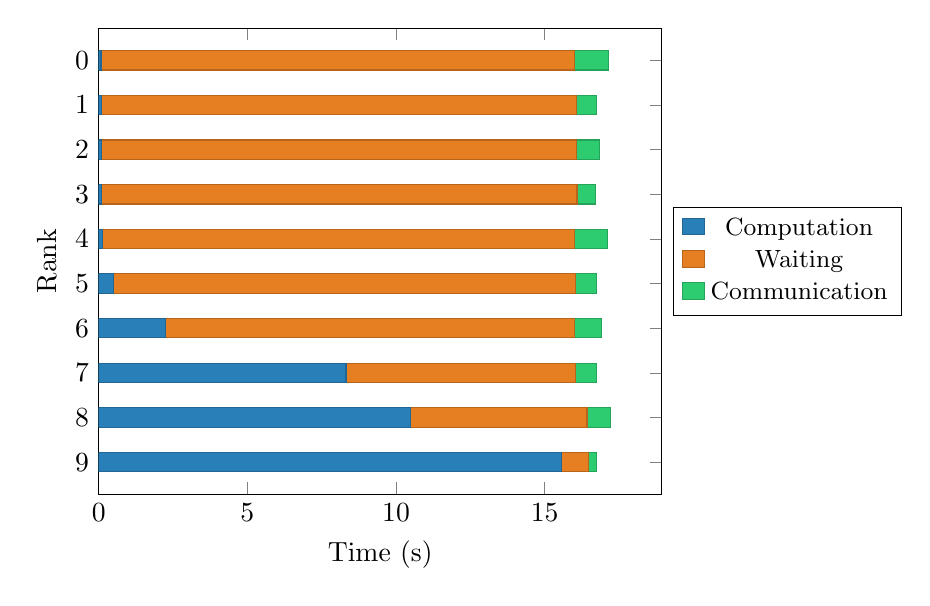
\begin{tikzpicture}
\begin{axis}[
    xbar stacked,
    bar width=7pt,
    y dir=reverse,
    ytick={0,...,9},
    xlabel={Time (s)},
    ylabel={Rank},
    legend style={at={(1.02,0.5)},anchor=west,font=\small},
    width=0.72\textwidth,
    height=7.5cm,
    xmin=0,
    enlarge y limits=0.08,
]
\addplot[fill=cWork,draw=cWork!80!black] coordinates {
    (0.075,0)(0.094,1)(0.079,2)(0.091,3)(0.125,4)
    (0.483,5)(2.253,6)(8.315,7)(10.496,8)(15.565,9)};
\addplot[fill=cWait,draw=cWait!80!black] coordinates {
    (15.936,0)(15.970,1)(15.999,2)(15.993,3)(15.867,4)
    (15.560,5)(13.751,6)(7.727,7)(5.926,8)(0.895,9)};
\addplot[fill=cComm,draw=cComm!80!black] coordinates {
    (1.134,0)(0.674,1)(0.756,2)(0.631,3)(1.129,4)
    (0.708,5)(0.897,6)(0.708,7)(0.788,8)(0.291,9)};
\legend{Computation,Waiting,Communication}
\end{axis}
\end{tikzpicture}
\caption{Per-rank timing breakdown for Task~1 (static block partitioning).}
\label{fig:task1_timing}
\end{figure}

Figure~\ref{fig:task1_timing} reveals extreme load imbalance. Rank~9,
which processes the rows closest to the real axis (where the Mandelbrot set
boundary lies), spends 15.6\,s computing, while ranks~0--4, assigned to the
top of the complex plane where most points escape quickly, compute for under
0.13\,s---a ratio exceeding 200$\times$.

The imbalance arises because the computational cost per pixel is highly
non-uniform: pixels near the set boundary require up to 1000 iterations,
whereas pixels far from the set escape in a handful. Block partitioning
assigns contiguous rows to each rank, concentrating the expensive pixels on
the ranks nearest the center. The resulting idle time (orange bars)
dominates the wall-clock time, wasting the parallel resources.

%======================================================================
\section{Task~2: Dynamic Decomposition (Master--Worker)}
\label{sec:task2}
%======================================================================

\subsection{Algorithm}

To address the load imbalance of block partitioning, a master--worker scheme
is used. Rank~0 acts as the master, distributing work to the $p{-}1 = 9$
workers in chunks of a tuneable \texttt{chunksize}. The protocol uses
point-to-point communication (no collectives):

\begin{enumerate}\itemsep0pt
\item The master sends each idle worker a starting index via \texttt{TAG\_WORK}.
\item The worker computes the iteration counts for \texttt{chunksize}
      consecutive pixels, then returns the starting index and results via
      \texttt{TAG\_RESULT}.
\item The master receives a result from \emph{any} worker
      (\texttt{MPI\_ANY\_SOURCE}), stores it, and either sends the next
      chunk or a termination signal (\texttt{TAG\_DONE}).
\item Workers loop until they receive \texttt{TAG\_DONE}.
\end{enumerate}

The implementation uses non-blocking communication (\texttt{MPI\_Isend},
\texttt{MPI\_Irecv}, \texttt{MPI\_Waitall}) to overlap the send of results
with the receipt of the next work assignment, reducing idle time.

Padding is applied so that $H + \text{pad}$ is divisible by
\texttt{chunksize}; out-of-bounds pixels are computed but not written to the
image.

\subsection{Key Code --- Master}
\begin{lstlisting}
idx = 0;  n_busy = 0;
for (r = 1; r < n_ranks && idx < half; r++) {
    MPI_Isend(&idx, 1, MPI_INT, r, TAG_WORK, comm, &req);
    n_busy++;  idx += chunksize;
}
while (idx < half || n_busy > 0) {
    MPI_Recv(&result_idx, 1, MPI_INT, MPI_ANY_SOURCE,
             TAG_RESULT, comm, &status);
    src = status.MPI_SOURCE;
    MPI_Irecv(&n[result_idx], chunksize, MPI_INT, src,
              TAG_RESULT, comm, &req);
    if (idx < half) {
        MPI_Isend(&idx, 1, MPI_INT, src, TAG_WORK, comm, &req2);
        idx += chunksize;
    } else {
        MPI_Isend(NULL,0,MPI_BYTE, src, TAG_DONE, comm, &req2);
        n_busy--;
    }
    MPI_Waitall(2, (MPI_Request[]){req, req2}, MPI_STATUSES_IGNORE);
}
\end{lstlisting}

\subsection{Key Code --- Worker}
\begin{lstlisting}
MPI_Recv(&idx, 1, MPI_INT, 0, MPI_ANY_TAG, comm, &status);
if (status.MPI_TAG == TAG_DONE) goto end;
while (1) {
    MPI_Irecv(&next_idx, 1, MPI_INT, 0, MPI_ANY_TAG, comm, &req_next);
    for (loop = 0; loop < chunksize; loop++) { /* compute */ }
    MPI_Isend(&idx,  1, MPI_INT, 0, TAG_RESULT, comm, &req1);
    MPI_Isend(_n, chunksize, MPI_INT, 0, TAG_RESULT, comm, &req2);
    MPI_Waitall(3, (MPI_Request[]){req_next,req1,req2}, statuses);
    if (statuses[0].MPI_TAG == TAG_DONE) break;
    idx = next_idx;
}
\end{lstlisting}

\subsection{Load Balancing at Chunksize $\approx 100{,}000$}

\begin{figure}[h]\centering
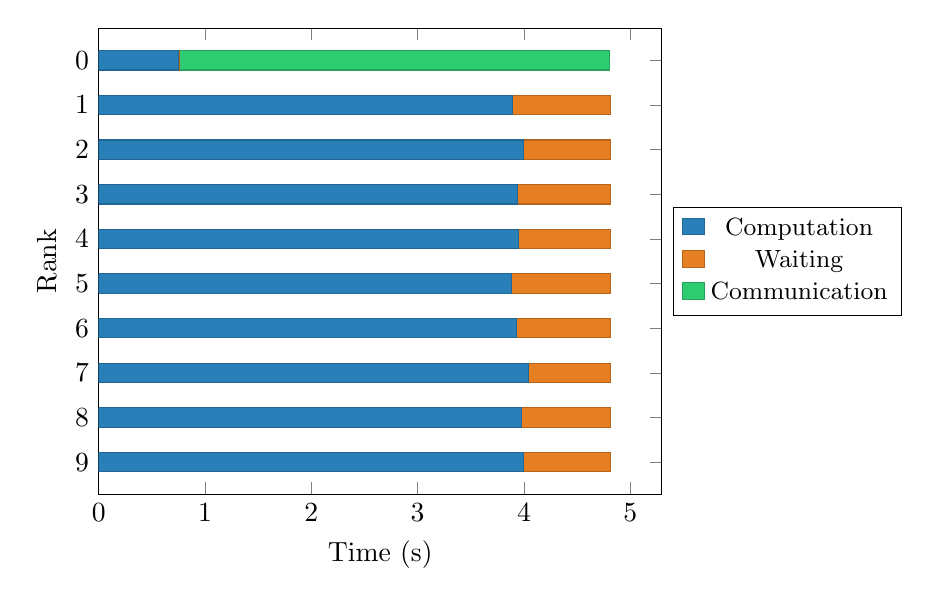
\begin{tikzpicture}
\begin{axis}[
    xbar stacked,
    bar width=7pt,
    y dir=reverse,
    ytick={0,...,9},
    xlabel={Time (s)},
    ylabel={Rank},
    legend style={at={(1.02,0.5)},anchor=west,font=\small},
    width=0.72\textwidth,
    height=7.5cm,
    xmin=0,
    enlarge y limits=0.08,
]
\addplot[fill=cWork,draw=cWork!80!black] coordinates {
    (0.753,0)(3.892,1)(3.996,2)(3.940,3)(3.946,4)
    (3.886,5)(3.927,6)(4.042,7)(3.978,8)(3.996,9)};
\addplot[fill=cWait,draw=cWait!80!black] coordinates {
    (0.008,0)(0.921,1)(0.817,2)(0.872,3)(0.867,4)
    (0.926,5)(0.885,6)(0.770,7)(0.834,8)(0.817,9)};
\addplot[fill=cComm,draw=cComm!80!black] coordinates {
    (4.048,0)(0.000,1)(0.000,2)(0.000,3)(0.000,4)
    (0.000,5)(0.000,6)(0.000,7)(0.001,8)(0.001,9)};
\legend{Computation,Waiting,Communication}
\end{axis}
\end{tikzpicture}
\caption{Per-rank timing for Task~2 (chunksize $\approx 100{,}000$, 10~MPI processes).}
\label{fig:task2_timing}
\end{figure}

Figure~\ref{fig:task2_timing} shows a dramatic improvement over Task~1.
All nine workers spend $3.89$--$4.04$\,s computing (a spread of only
$\pm 2\%$), with negligible communication overhead.
Workers that finish a cheap chunk quickly are immediately assigned another,
so the workload self-balances over many scheduling rounds.
The master (rank~0) performs little computation itself but spends 4.05\,s on
communication managing the work distribution.
The total wall-clock time is $4.81$\,s.

\subsection{Runtime vs.\ Chunksize}

\begin{figure}[h]\centering
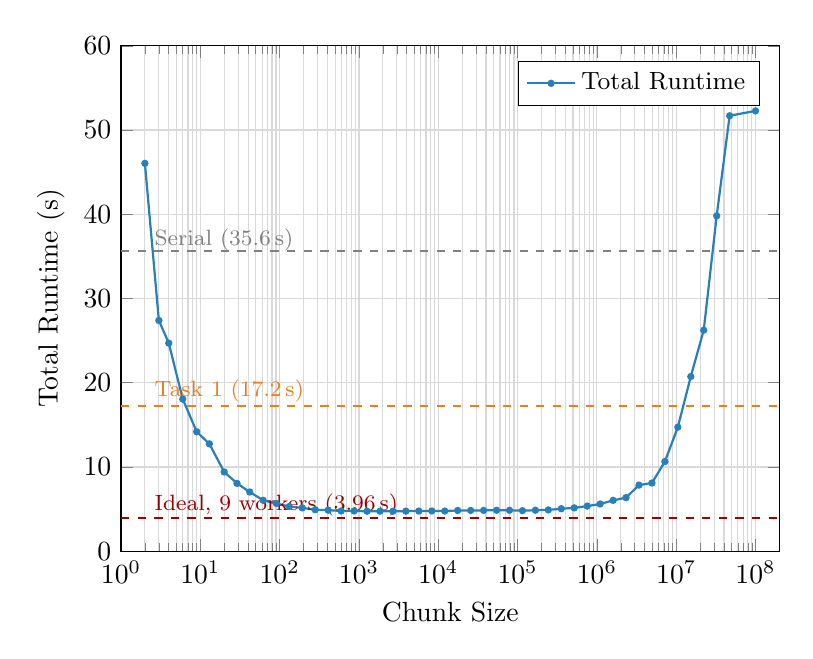
\begin{tikzpicture}
\begin{semilogxaxis}[
    xlabel={Chunk Size},
    ylabel={Total Runtime (s)},
    grid=both,
    grid style={gray!30},
    width=0.82\textwidth,
    height=8cm,
    xmin=1, xmax=2e8,
    ymin=0, ymax=60,
    legend style={at={(0.97,0.97)},anchor=north east,font=\small},
    every axis plot/.append style={thick},
]
\addplot[cWork,mark=*,mark size=0.9pt] coordinates {
    (2,46.049)(3,27.396)(4,24.701)(6,18.060)(9,14.180)
    (13,12.746)(20,9.404)(29,8.052)(42,7.027)(62,6.040)
    (91,5.663)(132,5.308)(193,5.144)(281,4.919)(409,4.874)
    (596,4.777)(868,4.774)(1264,4.743)(1842,4.748)
    (2682,4.743)(3906,4.756)(5689,4.767)(8286,4.777)
    (12067,4.769)(17575,4.837)(25595,4.838)(37275,4.845)
    (54286,4.865)(79060,4.858)(115139,4.813)(167683,4.864)
    (244205,4.901)(355648,5.044)(517947,5.140)(754312,5.356)
    (1098541,5.602)(1599858,6.033)(2329951,6.359)
    (3393221,7.848)(4941713,8.093)(7196856,10.639)
    (10481131,14.727)(15264179,20.735)(22229964,26.242)
    (32374575,39.812)(47148663,51.698)(100000000,52.275)
};
\addlegendentry{Total Runtime}
\addplot[dashed,gray,forget plot,domain=1:2e8] {35.632};
\node[anchor=west,font=\footnotesize,gray] at (axis cs:2,37) {Serial (35.6\,s)};
\addplot[dashed,red!60!black,forget plot,domain=1:2e8] {35.632/9};
\node[anchor=west,font=\footnotesize,red!60!black] at (axis cs:2,5.5) {Ideal, 9 workers (3.96\,s)};
\addplot[dashed,cWait,forget plot,domain=1:2e8] {17.21};
\node[anchor=west,font=\footnotesize,cWait] at (axis cs:2,19) {Task~1 (17.2\,s)};
\end{semilogxaxis}
\end{tikzpicture}
\caption{Total runtime vs.\ chunksize for Task~2 with 9~workers. Reference
lines show the serial time, ideal parallel time, and Task~1 block-partitioning time.}
\label{fig:task2_chunksize}
\end{figure}

Figure~\ref{fig:task2_chunksize} exhibits three regimes:

\begin{itemize}\itemsep2pt
\item \textbf{Small chunksize ($< 100$):} Communication overhead
    dominates. Each chunk requires a round-trip of MPI messages, so
    $\sim H / C$ message exchanges occur. At chunksize~2, the runtime
    exceeds even the serial baseline.

\item \textbf{Optimal range ($\sim 500$--$100{,}000$):} The runtime
    plateaus near $4.75$\,s (speedup $\approx 7.5\times$).
    Communication cost per chunk is amortised over enough computation,
    and chunks are small enough that dynamic scheduling balances the load
    effectively. The optimum is broadly flat, making the method robust to
    the choice of chunksize within this range.

\item \textbf{Large chunksize ($> 10^6$):} With fewer, bigger chunks the
    scheduling degenerates toward static block partitioning. Load
    imbalance re-emerges and the runtime climbs steeply. At
    $C = H \approx 1.1 \times 10^8$, a single worker performs all the
    work and the runtime approaches the serial time.
\end{itemize}

\subsection{Comparison with Task~1}

When the chunksize equals one-tenth of the total work
($H/10 = 11{,}251{,}500$), each of the 9~workers receives a large,
contiguous block. The data at $C = 10{,}481{,}131$ gives a wall-clock time
of $14.7$\,s, comparable to Task~1's $17.2$\,s. The per-rank profile at
this chunksize (not shown) exhibits the same pattern as Task~1:
ranks assigned to the centre of the complex plane compute for
$\sim 14$\,s while ranks at the edges finish in under $0.1$\,s.
This confirms that large-chunksize dynamic scheduling recovers the
load-imbalanced behaviour of block partitioning.

The small discrepancy (14.7\,s vs.\ 17.2\,s) arises because the fastest
worker finishes its first chunk quickly and receives a second one,
providing a degree of dynamic rebalancing that pure block partitioning
cannot.

%======================================================================
\section{Task~3: Static Decomposition (Cyclic Partitioning)}
\label{sec:task3}
%======================================================================

\subsection{Data Distribution and Algorithm}

Cyclic (round-robin) partitioning assigns pixel $i$ to rank $(i \bmod p)$.
This interleaves the workload across all rows of the grid so that each rank
processes a mix of cheap and expensive pixels, naturally balancing the load.

The implementation constructs an interleaved index array on the root:
\begin{lstlisting}
for (idx = 0; idx < chunksize; idx++)
    for (blk = 0; blk < n_ranks; blk++)
        n[c++] = blk * chunksize + idx;
\end{lstlisting}
\texttt{MPI\_Scatter} distributes $C$ consecutive elements from this array
to each rank, so rank~$r$ receives the indices
$\{r C,\, r C{+}1,\, \ldots\}$ in the interleaved order, which correspond
to every $p$-th pixel in the original domain.

After computation and \texttt{MPI\_Gather}, the root reverses the cyclic
permutation to reconstruct the image in scan-line order:
\begin{lstlisting}
for (idx = 0; idx < chunksize; idx++)
    for (blk = 0; blk < n_ranks; blk++) {
        loop = blk * chunksize + idx;
        x[loop] = logf((float)n[c++]) * inv_log_maxiter;
    }
\end{lstlisting}

\subsection{Performance}

\begin{table}[h]\centering
\begin{tabular}{@{}lccc@{}}
\toprule
 & Wall-clock (s) & Speedup & Ideal ($f{\approx}0$) \\
\midrule
Block  (Task~1) & 17.21 & 2.07$\times$ & 10$\times$ \\
Cyclic (Task~3) &  4.46 & 7.99$\times$ & 10$\times$ \\
\bottomrule
\end{tabular}
\caption{Comparison of static block and cyclic partitioning.}
\label{tab:task3}
\end{table}

\subsection{Load Balancing}

\begin{figure}[h]\centering
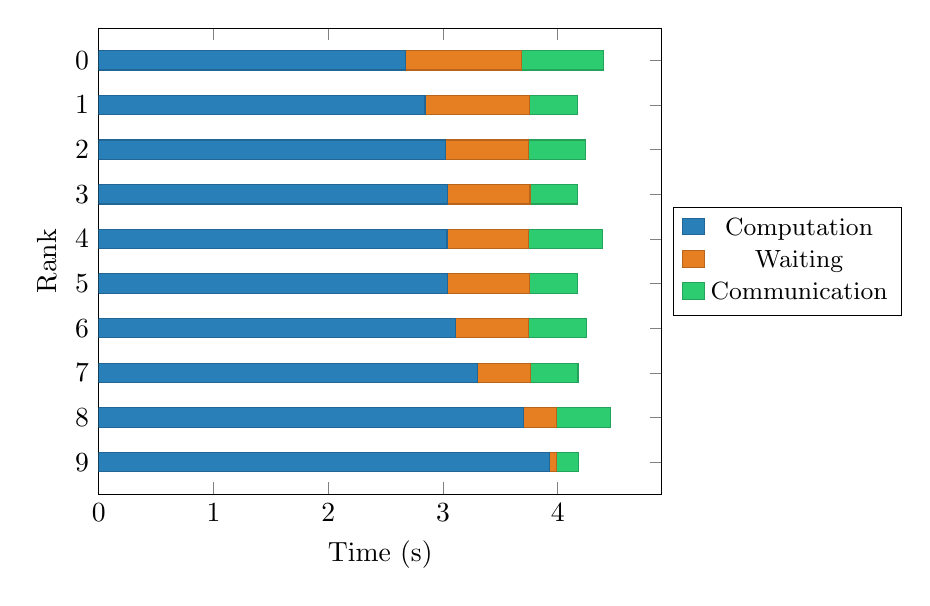
\begin{tikzpicture}
\begin{axis}[
    xbar stacked,
    bar width=7pt,
    y dir=reverse,
    ytick={0,...,9},
    xlabel={Time (s)},
    ylabel={Rank},
    legend style={at={(1.02,0.5)},anchor=west,font=\small},
    width=0.72\textwidth,
    height=7.5cm,
    xmin=0,
    enlarge y limits=0.08,
]
\addplot[fill=cWork,draw=cWork!80!black] coordinates {
    (2.676,0)(2.844,1)(3.019,2)(3.041,3)(3.035,4)
    (3.041,5)(3.113,6)(3.304,7)(3.704,8)(3.931,9)};
\addplot[fill=cWait,draw=cWait!80!black] coordinates {
    (1.006,0)(0.914,1)(0.725,2)(0.718,3)(0.707,4)
    (0.717,5)(0.632,6)(0.456,7)(0.282,8)(0.062,9)};
\addplot[fill=cComm,draw=cComm!80!black] coordinates {
    (0.715,0)(0.415,1)(0.502,2)(0.417,3)(0.649,4)
    (0.418,5)(0.508,6)(0.417,7)(0.474,8)(0.185,9)};
\legend{Computation,Waiting,Communication}
\end{axis}
\end{tikzpicture}
\caption{Per-rank timing breakdown for Task~3 (static cyclic partitioning).}
\label{fig:task3_timing}
\end{figure}

\subsection{Comparison with Block Partitioning}

Figure~\ref{fig:task3_timing} shows a strikingly more balanced workload
than Task~1 (Figure~\ref{fig:task1_timing}). Computation times range from
2.68\,s (rank~0) to 3.93\,s (rank~9)---a ratio of just $1.47\times$,
compared to over $200\times$ for block partitioning.

A residual gradient remains because the cyclic interleaving is not perfectly
uniform: rank~9 receives the last pixel from each ``round,'' which
systematically biases it toward rows closer to the set boundary. However,
this effect is minor and the waiting times (orange bars) are much shorter
than in Task~1.

The speedup improves from $2.07\times$ (block) to $7.99\times$ (cyclic)
with the same communication pattern (one \texttt{Scatter} + one
\texttt{Gather}). The improvement is entirely due to better load
distribution.

%======================================================================
\section{Conclusions}
\label{sec:conclusions}
%======================================================================

\begin{table}[h]\centering
\begin{tabular}{@{}lcccc@{}}
\toprule
Method & Runtime (s) & Speedup & Work Ratio & Efficiency \\
\midrule
Serial               & 35.63 & ---           & ---           & --- \\
Block (Task~1)       & 17.21 & $2.07\times$  & $207\times$   & 20.7\% \\
Dynamic (Task~2)     &  4.76 & $7.49\times$  & $1.04\times$  & 83.3\%$^\dagger$ \\
Cyclic (Task~3)      &  4.46 & $7.99\times$  & $1.47\times$  & 79.9\% \\
\bottomrule
\end{tabular}\\[4pt]
{\footnotesize $^\dagger$\,Efficiency relative to 9~computing workers.
Relative to all 10 processes: 74.9\%.}
\caption{Summary comparison of all three methods at $N = 15{,}000$.
Work Ratio = max(work) / min(work) across worker ranks.}
\label{tab:summary}
\end{table}

\paragraph{Block partitioning} is the simplest to implement (one
\texttt{Scatter} + one \texttt{Gather}) but performs poorly on workloads
with spatial non-uniformity, as is the case for the Mandelbrot set. Its
speedup of $2.07\times$ with 10~processes represents a parallel efficiency
of only 21\%.

\paragraph{Dynamic scheduling} achieves near-ideal load balance (work-time
spread $< 4\%$) and a speedup of $7.49\times$. Its robustness to workload
irregularity makes it the most generally applicable strategy. The cost is
added code complexity and the dedication of one process to scheduling. The
optimal chunksize lies in a broad plateau ($\sim 500$--$100{,}000$), making
it easy to tune. For very small chunks communication overhead dominates; for
very large chunks load imbalance re-emerges.

\paragraph{Cyclic partitioning} delivers the highest speedup
($7.99\times$) with the same simplicity as block partitioning. It succeeds
because the Mandelbrot workload varies \emph{smoothly} across the grid;
interleaving ensures each rank samples all regions evenly. Unlike dynamic
scheduling, all 10~processes contribute to computation.

\paragraph{Recommendation.} For the Mandelbrot problem, \textbf{cyclic
partitioning is the best strategy}: it combines the highest speedup, lowest
implementation complexity, and minimal communication overhead. Dynamic
scheduling would be preferable for workloads with less predictable
structure, where static interleaving cannot guarantee balance.

\end{document}
